\begin{figure*}[b!]
\centering
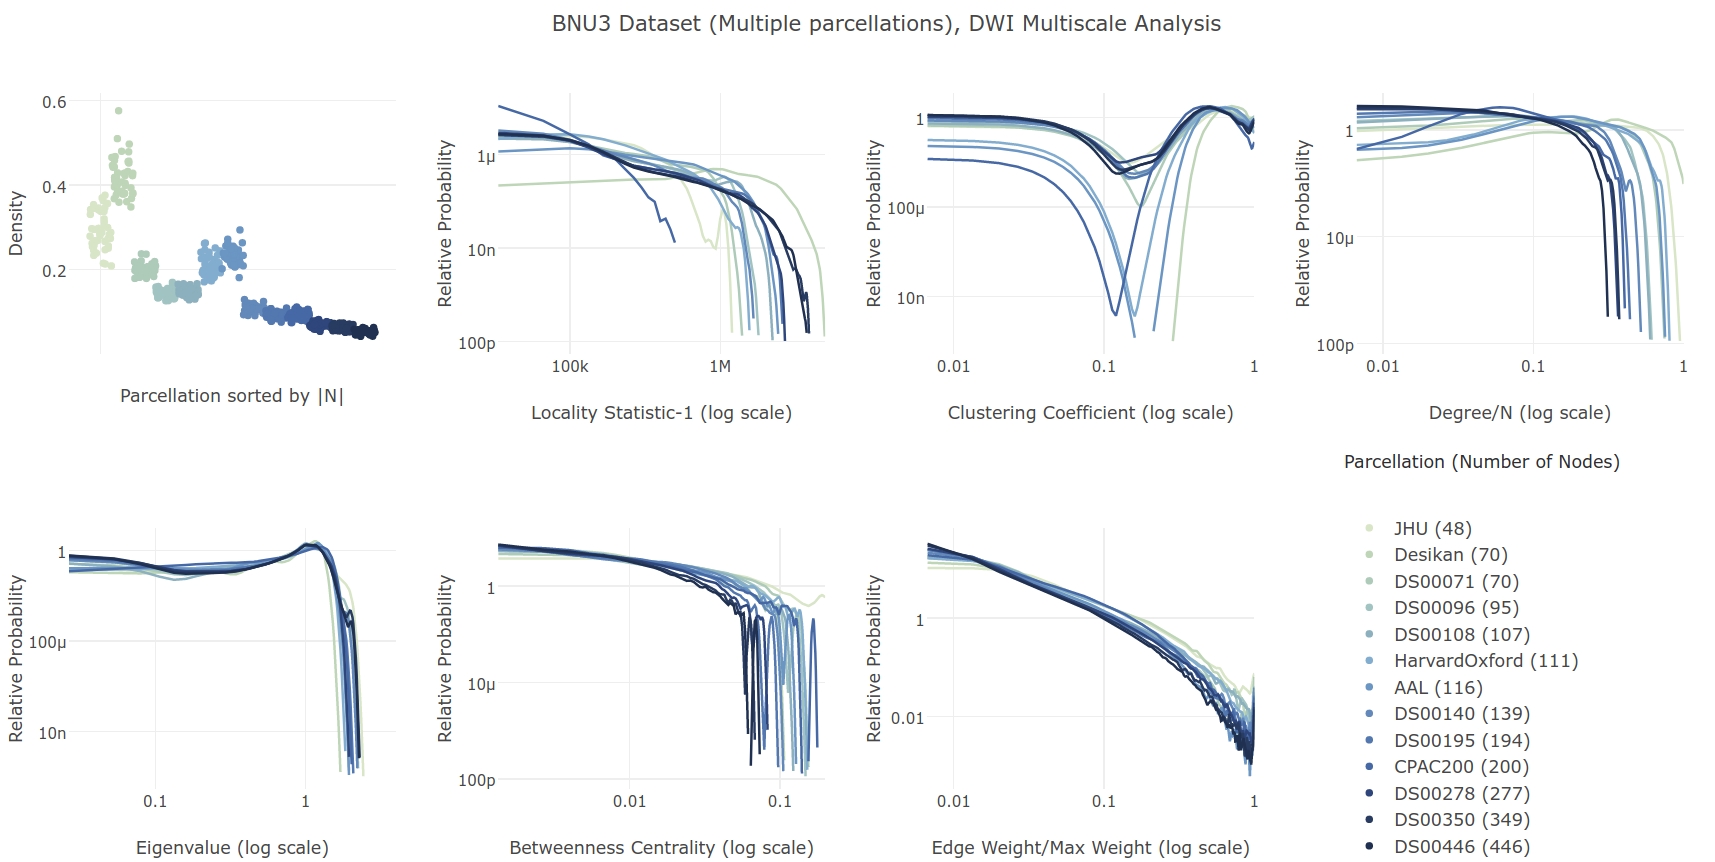
\includegraphics[width=\textwidth]{./figs/fig_multiscale.png}
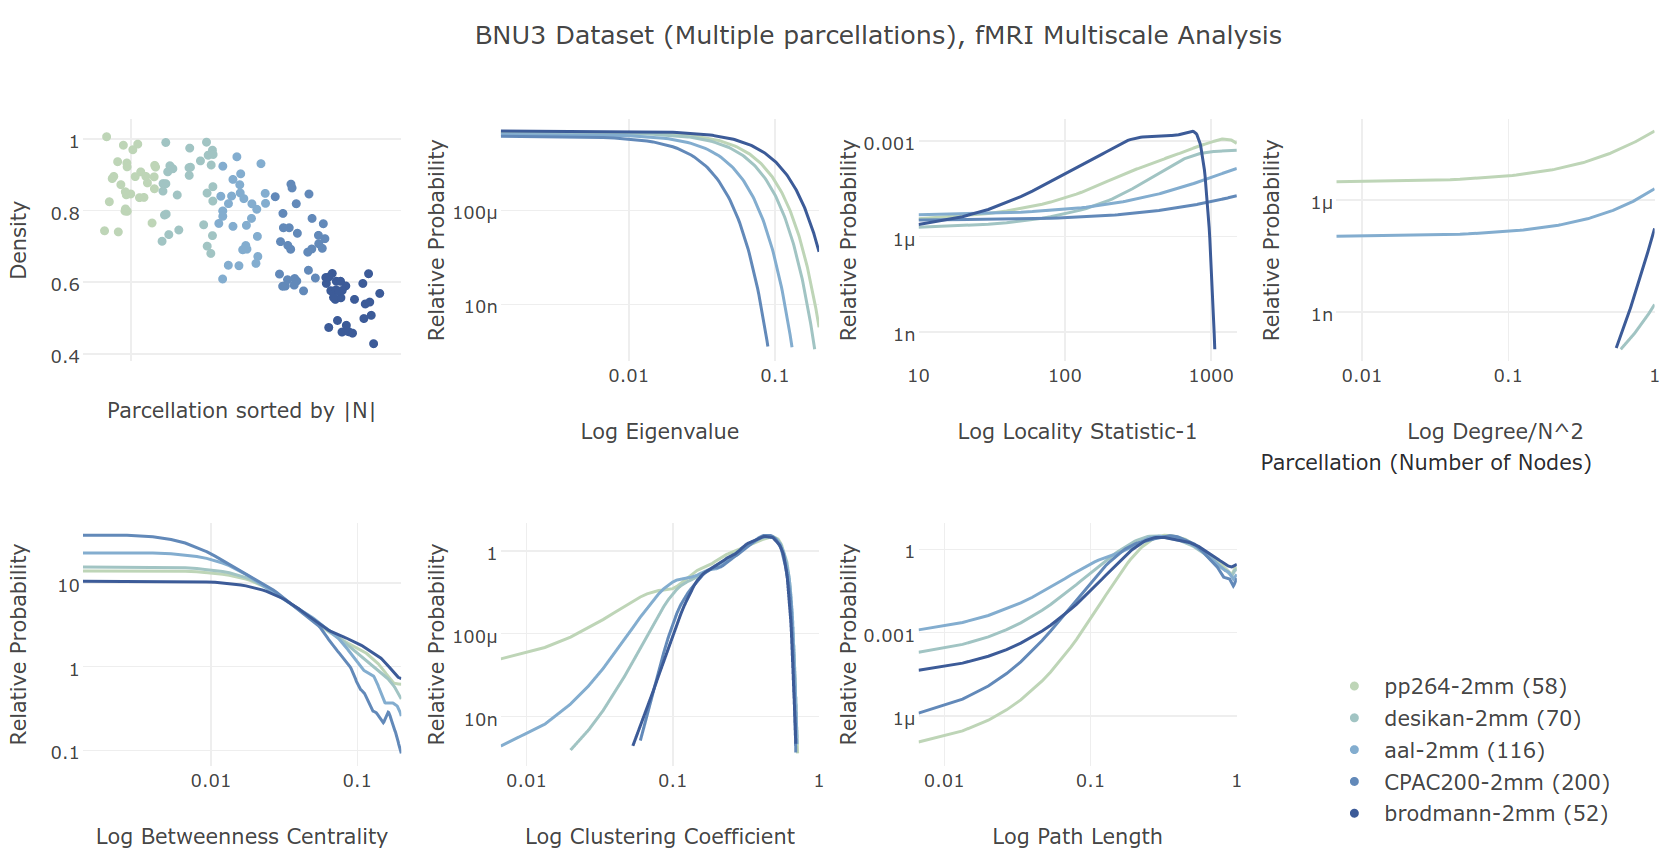
\includegraphics[width=\textwidth]{./figs/fig_fmri_multiscale.png}
\caption{\textbf{Multi-Scale Connectome Analysis.}
\ndmg~produces connectomes at a variety of scales, enabling investigation
of graph properties between parcellation schemes. We can observe that the statistics are qualitatively similar in shape
across scales, however, they are quantitatively significantly different, for both the diffusion (top) and functional (bottom) connectomes. This suggests that claims made or analyses
performed on a given scale may not hold when applied to another scale. This is impactful, as the choice of parcellation
has significant bearing on the results of a scientific study.}
% @gk: why don't we have ipsi-lateral and contra-lateral broken out here?
% @gk: i don't understand from the text what the curves are.  are they averages over subjects within this group? if so, specify.
\label{fig:multiscale}
\end{figure*}